\documentclass[10pt,aspectratio=169]{beamer}

% ---------- Theme ----------
\usetheme{Madrid}
\usepackage[T1]{fontenc}
\usepackage[utf8]{inputenc}
\usepackage{amsmath,amssymb}
\usepackage{booktabs}
\usepackage{graphicx}
\usepackage{xcolor}
\usepackage{tikz}
\usepackage{pgfplots}
\pgfplotsset{compat=1.18}

% Colors (works with or without metropolis)
\definecolor{accent}{HTML}{2563EB}
\definecolor{accent2}{HTML}{DC2626}
\definecolor{accent3}{HTML}{059669}
\definecolor{good}{HTML}{059669}
\definecolor{bad}{HTML}{DC2626}

\setbeamercolor{frametitle}{bg=accent,fg=white}
\setbeamercolor{title separator}{fg=accent}
\setbeamercolor{progress bar}{fg=accent}

% Compact spacing
\setbeamertemplate{itemize item}{\textcolor{accent}{$\bullet$}}
\setbeamertemplate{itemize subitem}{\textcolor{accent}{$\circ$}}

% ---------- Title ----------
\title{Mortgage Prepayment Risk Modeling}
\subtitle{From Kaplan--Meier to Deep Survival Analysis}
\author{Rose Lin, Paolo Smalhout, Daniel Tuzes}
\institute{MTH 9877 --- Interest Rate and Credit Models\\Baruch College, Spring 2026}
\date{May 13, 2026}

% =========================================================================
\begin{document}

% ============================================================ Slide 1: Title
\begin{frame}[plain]
    \titlepage
\end{frame}

% ============================================================ Slide 2: Outline / Project Scope
\begin{frame}{Project Scope}

    \textbf{Goal.} Build a survival-analysis pipeline for mortgage prepayment on Freddie Mac single-family data, comparing classical, ML, and deep-learning approaches.

    \vspace{0.6em}

    \textbf{What we implemented:}
    \begin{itemize}\itemsep2pt
        \item \textbf{Part A.} Kaplan--Meier survival on the full 31.7M-loan population, stratified by FICO/LTV/vintage/purpose
        \item \textbf{Part B.} Cox proportional hazards (origination + vintage-macro covariates), PH diagnostics
        \item \textbf{Part C.} ML models (LogReg, RF, LightGBM) for horizon-specific prepayment prediction; Cox baseline
        \item \textbf{Part D.} Deep Cox model (DeepSurv) + linear-Cox-via-SGD ablation
    \end{itemize}

    \vspace{0.6em}

    \textbf{Headline result.} Deep Cox: AUC = 0.729 at T=60 vs 0.685 for the matched-architecture linear baseline. Gap widens monotonically with horizon: $+0.003$ at T=12 $\to$ $+0.045$ at T=60.

\end{frame}

% ============================================================ Slide 3: Data
\begin{frame}{Data: Freddie Mac Single-Family Loan-Level}

    \textbf{Population.} 31{,}688{,}129 30-year fixed-rate mortgages, originated 1999--2025.

    \vspace{0.6em}

    \textbf{Outcomes (cause-specific framing for prepayment):}
    \begin{itemize}\itemsep1pt
        \item Prepaid (Zero Balance Code 01): 21{,}748{,}774 (68.6\%) --- the event
        \item Credit-related termination (ZBC 03, 09): 532{,}230 (1.7\%)
        \item Other termination (ZBC 02, 15, 16, 96): 265{,}311 (0.8\%)
        \item Right-censored (still active): 9{,}141{,}814 (28.8\%)
    \end{itemize}

    \vspace{0.6em}

    \textbf{Survival table.} One row per loan with \texttt{Duration}, \texttt{Event\_Prepay}, and 39 origination covariates. Built once via polars, persisted to parquet. Sentinel codes (DTI=999, MI=999, Credit=9999) cleaned to NaN.

    \vspace{0.6em}

    \textbf{Train/test split.} By vintage --- train: $\leq$ 2014 (full crisis cycle); test: 2015--2019. Single \texttt{canonical\_split.parquet} is the source of truth shared by Parts C and D.

\end{frame}

% ============================================================ Slide 4: Pipeline architecture
\begin{frame}{Pipeline Architecture}

    \textbf{Six scripts + four plotting notebooks, end-to-end $\approx 50$ minutes on CPU.}

    \vspace{0.5em}

    \begin{center}
        \small
        \begin{tabular}{lll}
            \toprule
            Stage                                   & Output                            & Runtime \\
            \midrule
            \texttt{build\_survival\_table.py}      & \texttt{survival\_table.parquet}  & 8 min   \\
            \texttt{part\_a\_survival\_analysis.py} & \texttt{results\_a/*.parquet}     & 3.5 min \\
            \texttt{part\_b\_cox\_model.py}         & \texttt{results\_b/*.parquet}     & 12 min  \\
            \texttt{part\_c\_ml\_models.py}         & \texttt{results\_cd/*.parquet}    & 12 min  \\
            \texttt{part\_d\_deep\_cox.py}          & \texttt{results\_cd/D\_*.parquet} & 19 min  \\
            \bottomrule
        \end{tabular}
    \end{center}

    \vspace{0.7em}

    \textbf{Design principle: compute / plot separation.}
    \begin{itemize}\itemsep1pt
        \item Scripts emit parquet only; no plotting in compute scripts.
        \item Plotting notebooks live alongside their parquets and read from \texttt{.}.
        \item A central \texttt{utilities.py} hosts the canonical pre-processing functions (\texttt{build\_feature\_matrix}, \texttt{build\_horizon\_targets}, \texttt{standardize\_three}) used by all parts.
    \end{itemize}

    \textbf{Reproducibility.} Single-source-of-truth split; encoders fit once on train, persisted; deterministic seeds throughout.

\end{frame}

% ============================================================ Slide 5: Part A overall KM
\begin{frame}{Part A --- Kaplan--Meier on the Full Population}

    \textbf{No sampling: KM fit on all 31.7M loans.}

    \begin{columns}[T,onlytextwidth]
        \column{0.55\textwidth}
        \begin{center}
            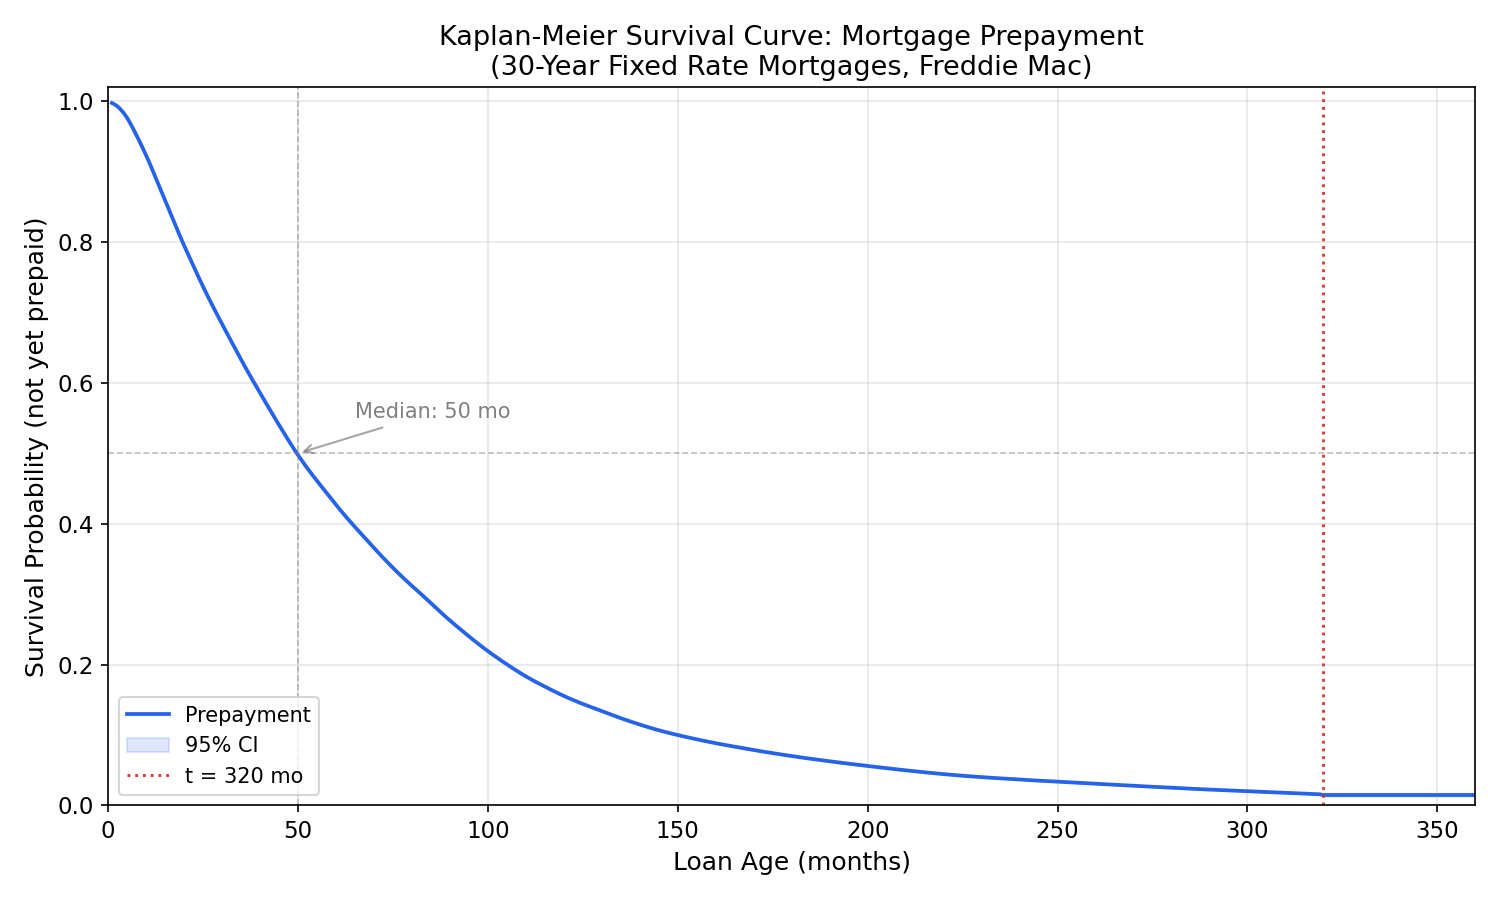
\includegraphics[width=\linewidth]{plots/A_km_overall.png}
        \end{center}

        \column{0.45\textwidth}
        \textbf{Key timepoints:}
        \vspace{0.3em}
        \small
        \begin{tabular}{rcc}
            \toprule
            $t$ (mo) & $S(t)$ & \% prepaid \\
            \midrule
            12       & 0.898  & 10.2       \\
            36       & 0.623  & 37.7       \\
            60       & 0.427  & 57.3       \\
            120      & 0.155  & 84.5       \\
            240      & 0.037  & 96.3       \\
            \bottomrule
        \end{tabular}

        \vspace{0.6em}
        \normalsize
        Median time to prepayment: \textbf{50 months}.

    \end{columns}

    \vspace{0.7em}

    \textbf{All non-prepay outcomes pooled as right-censored} (cause-specific framing): 9.94M censored vs 21.75M events.

\end{frame}

% ============================================================ Slide 6: Part A hazards
\begin{frame}{Part A --- Hazards}

    \begin{center}
        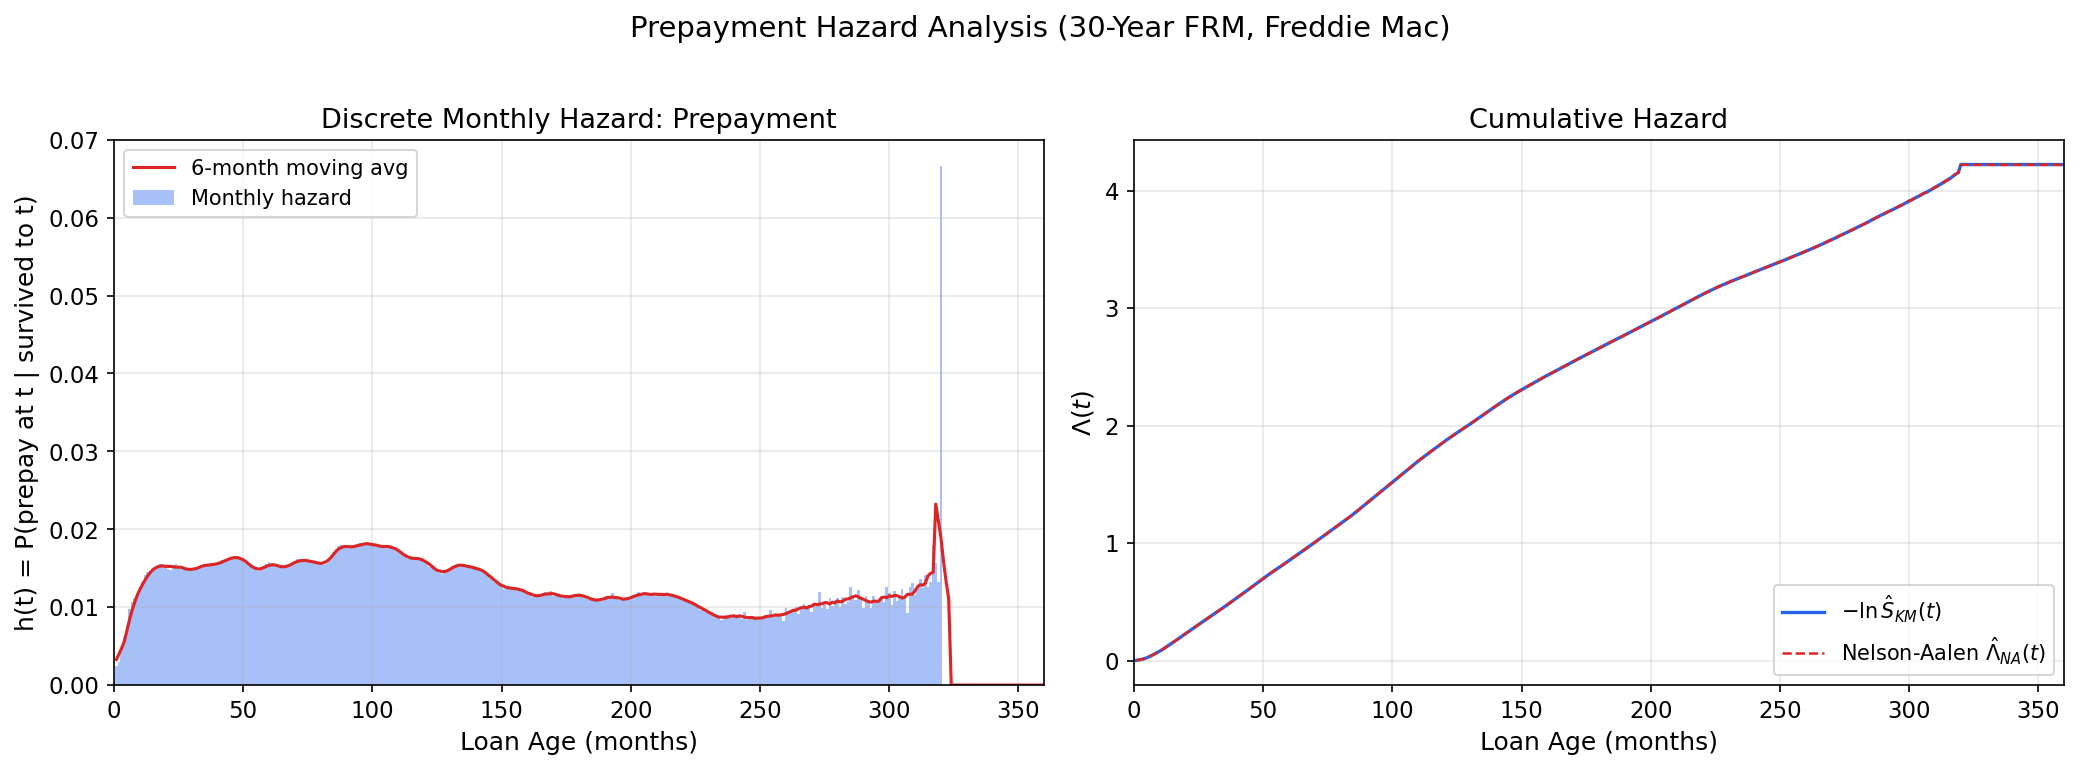
\includegraphics[width=0.65\linewidth]{plots/A_hazard_overall.png}
    \end{center}

    \textbf{Discrete monthly hazard:} ramps from $\approx$ 1\% at $t{=}6$ to $\approx$ 1.4\% at $t{=}12$, then plateaus at 1.5--1.7\% (annualized $\approx$ 17--18\%) from year 2 onward.

    \textbf{Sanity check:} $-\log S_{\text{KM}}$ vs Nelson--Aalen cumulative hazard agree to within numerical precision (as expected --- both estimate $H(t)$).

\end{frame}

% ============================================================ Slide 7: Part A stratification
\begin{frame}{Part A --- Stratification by Vintage and FICO}

    \begin{columns}[T,onlytextwidth]
        \column{0.5\textwidth}
        \begin{center}
            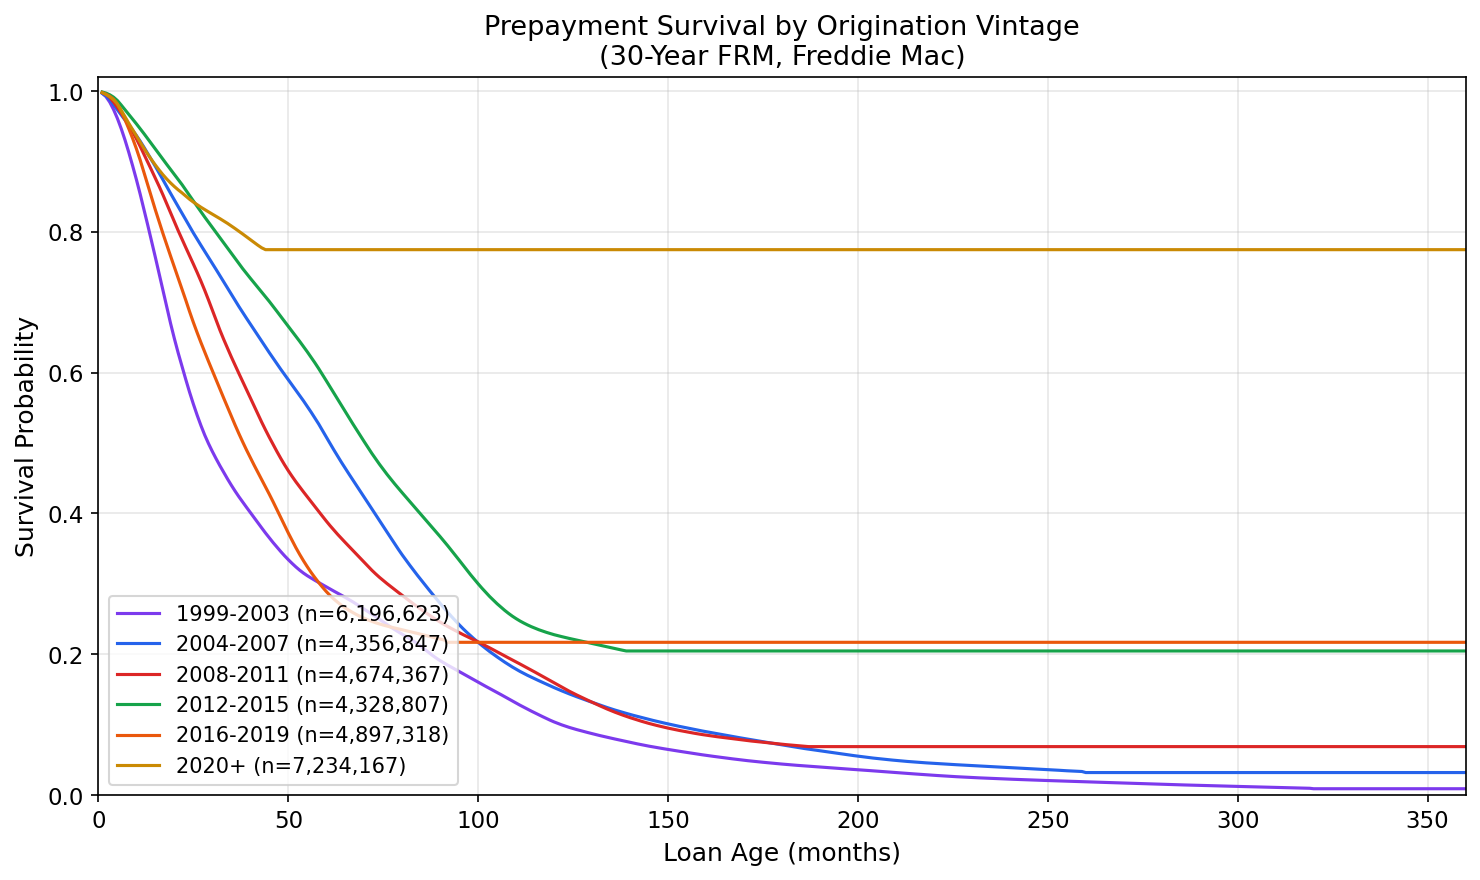
\includegraphics[width=\linewidth]{plots/A_km_by_vintage.png}
        \end{center}
        \small
        \textbf{Vintage dominates.}
        1999--2003: 96\% prepay, median 29 mo (post-2000 rate cuts).
        2020+: only 16\% prepay, median undefined (high-rate environment, recent vintages).

        \column{0.5\textwidth}
        \begin{center}
            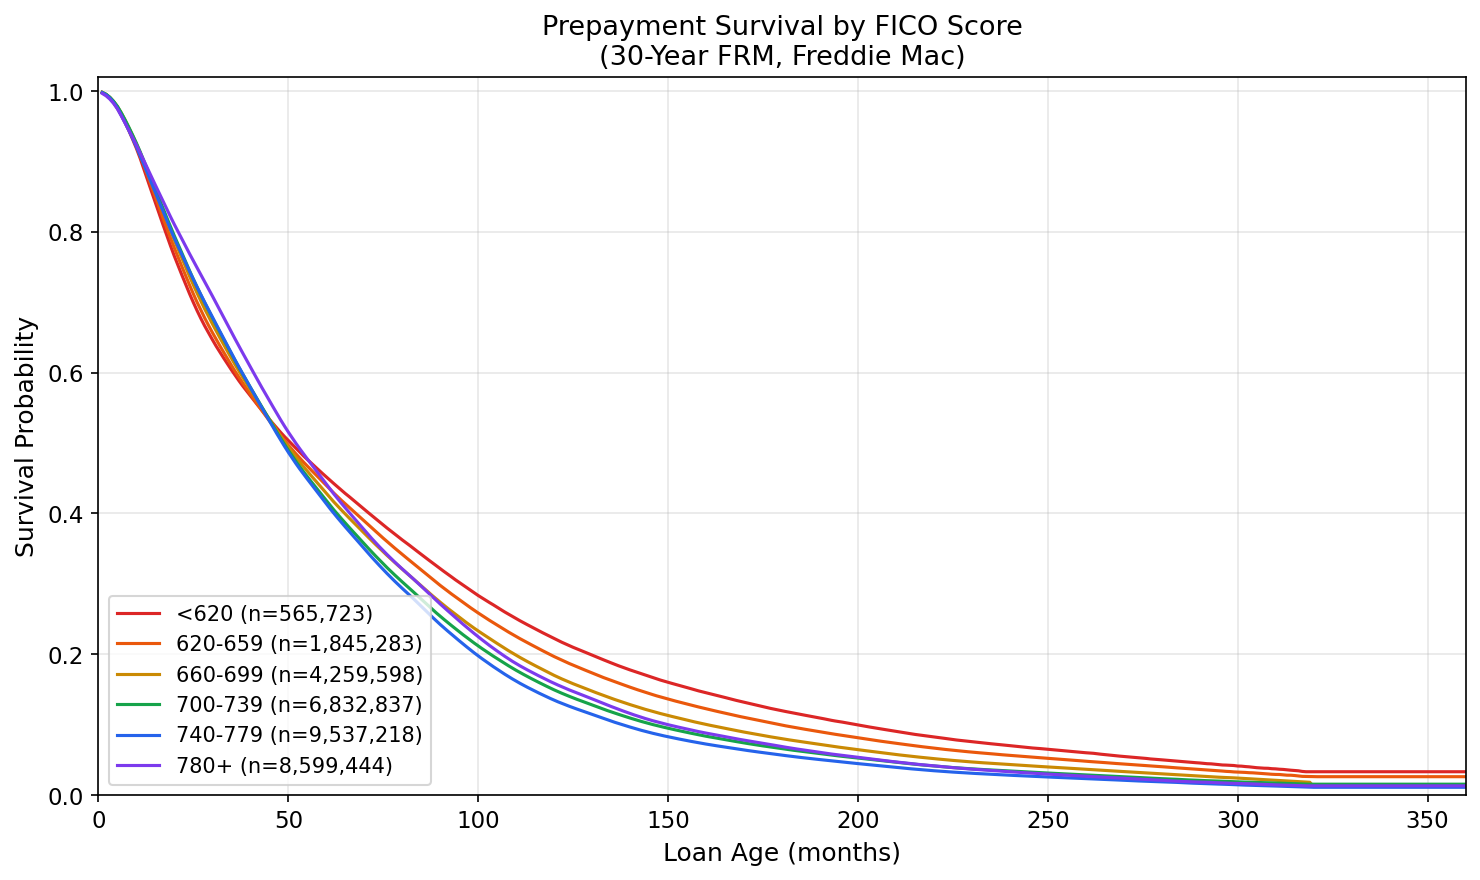
\includegraphics[width=\linewidth]{plots/A_km_by_fico.png}
        \end{center}
        \small
        \textbf{FICO is monotone but modest.}
        Prepay rate ranges from 78\% (sub-620) to 65\% (780+). Higher-FICO borrowers prepay less in proportion --- they often refinance into shorter-term loans, which exit the 30y FRM population sooner.

    \end{columns}

\end{frame}

% ============================================================ Slide 8: Part B base Cox
\begin{frame}{Part B --- Cox PH with Origination Covariates}

    \textbf{Base model.} 5\% sample (1.58M loans, 1.08M events), 15 origination covariates, lifelines + $\ell_2$ penalizer 0.001.

    \textbf{Concordance index: 0.6257}.

    \vspace{0.5em}

    \begin{columns}[T,onlytextwidth]
        \column{0.55\textwidth}
        \textbf{Largest hazard ratios:}
        \begin{itemize}\itemsep1pt
            \small
            \item \textbf{Original interest rate} (z): $\text{HR} = 1.58$ \\
                  \textit{the dominant driver --- high-rate borrowers refi when rates fall}
            \item \textbf{Original UPB} (z): $\text{HR} = 1.29$
            \item \textbf{Investment property}: $\text{HR} = 0.80$ \\
                  \textit{investors prepay less}
            \item \textbf{DTI missing}: $\text{HR} = 0.82$ \\
                  \textit{Relief Refinance flag (FAQ Q67)}
            \item \textbf{FICO} (z): $\text{HR} = 1.11$
        \end{itemize}

        \column{0.42\textwidth}
        \begin{center}
            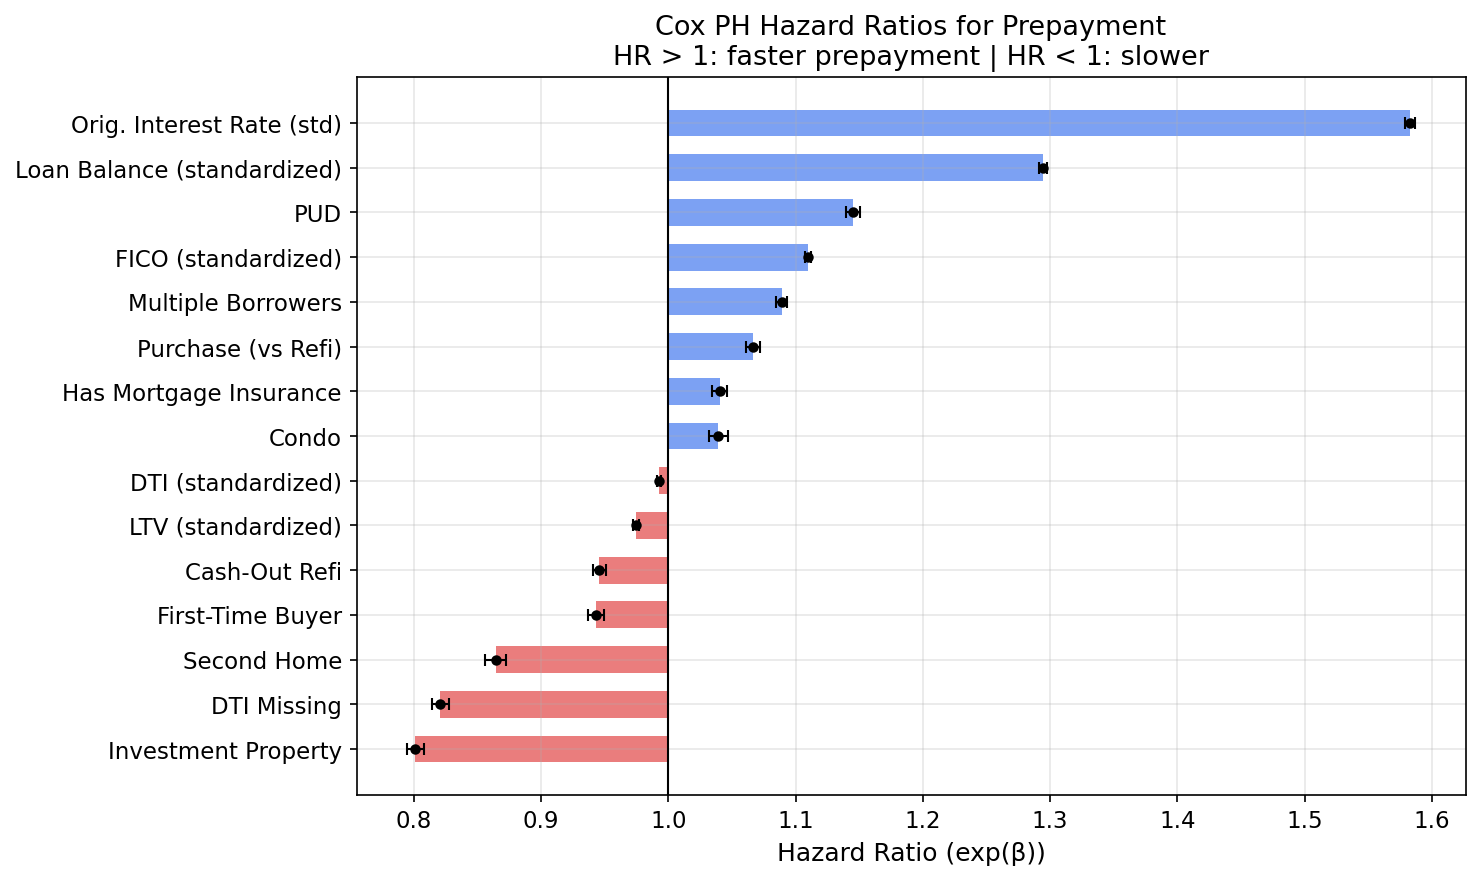
\includegraphics[width=\linewidth]{plots/B_hazard_ratios_base.png}
        \end{center}

    \end{columns}

\end{frame}

% ============================================================ Slide 9: Part B macro extension
\begin{frame}{Part B --- Vintage-Macro Extension}

    \textbf{Macro covariates joined at \texttt{FirstPaymentDate}} (origination): MortgageRate, 10y Treasury, Unemployment, HPI YoY.

    \textbf{Concordance: 0.6428 ($\Delta C = +0.017$, $\Delta\text{AIC} = -28{,}510$).}

    \vspace{0.5em}

    \begin{columns}[T,onlytextwidth]
        \column{0.55\textwidth}
        \textbf{Macro hazard ratios:}
        \begin{itemize}\itemsep1pt
            \small
            \item \textbf{10y Treasury at origination}: $\text{HR} = 0.78$
            \item \textbf{HPI YoY at origination}: $\text{HR} = 0.89$
            \item \textbf{Unemployment at origination}: $\text{HR} = 0.89$
            \item \textbf{30y mortgage rate at origination}: $\text{HR} = 0.94$
        \end{itemize}

        \vspace{0.5em}

        \textbf{Caveat:} these are vintage-macro covariates --- the macro state \emph{when the loan was originated}, not time-varying through the loan's life. A truly dynamic Cox would need the loan-month panel.

        \column{0.42\textwidth}
        \begin{center}
            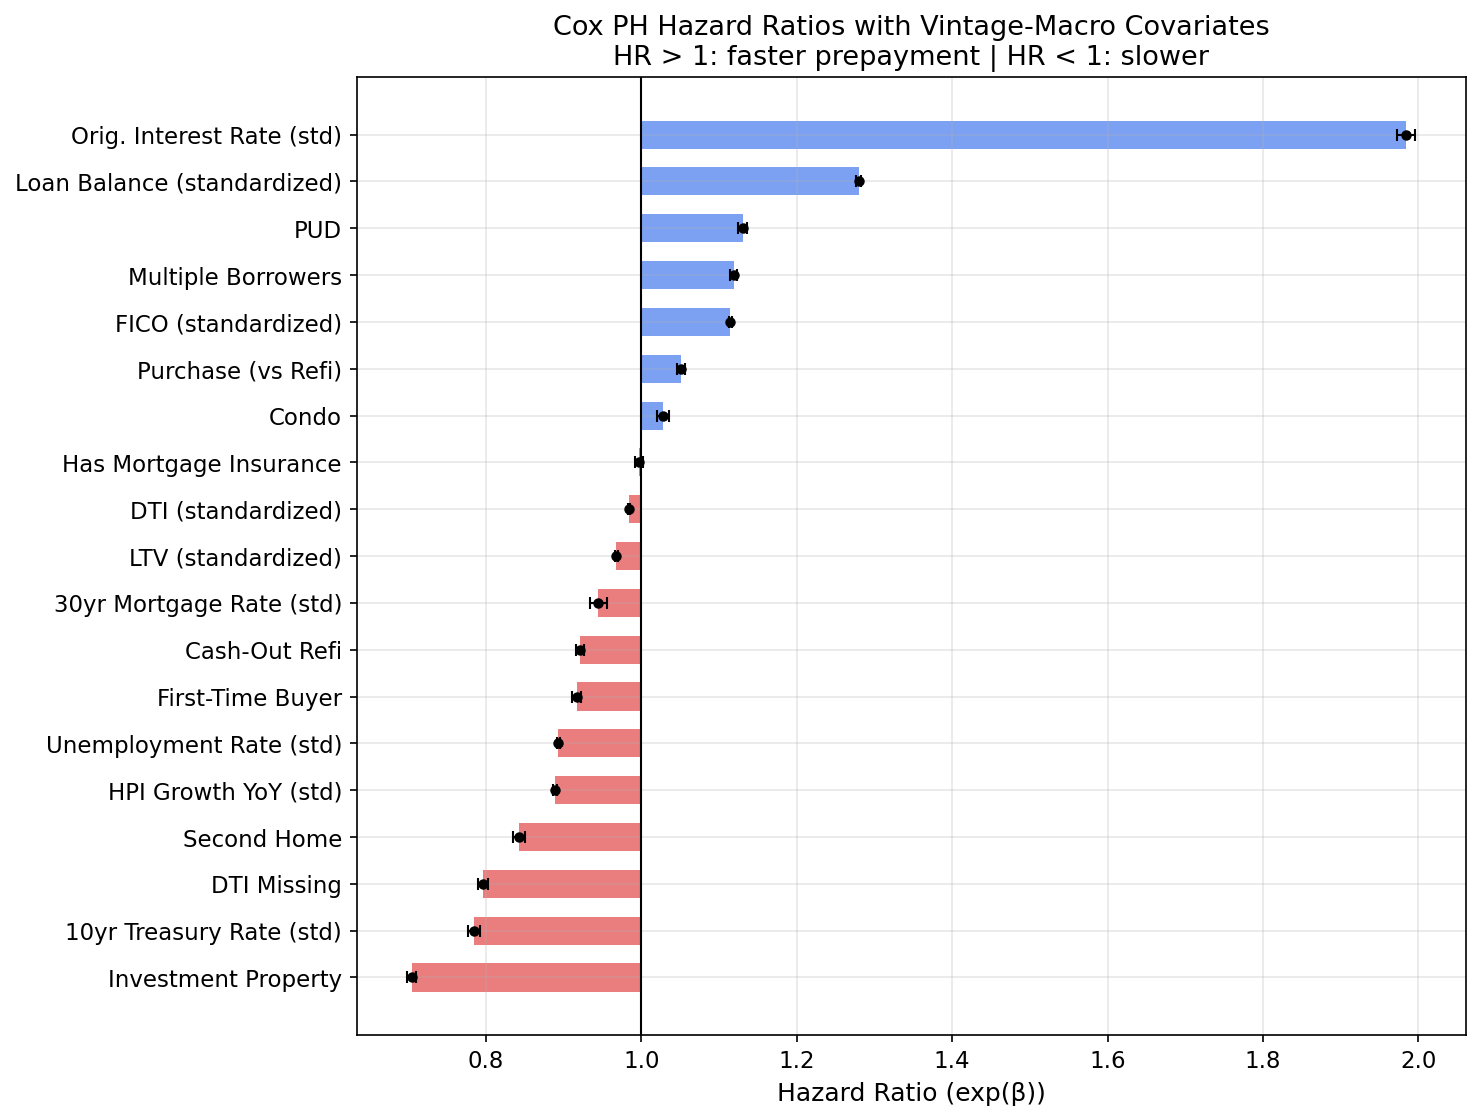
\includegraphics[width=\linewidth]{plots/B_hazard_ratios_macro.png}
        \end{center}
    \end{columns}

\end{frame}

% ============================================================ Slide 10: Part B PH diagnostics
\begin{frame}{Part B --- Proportional Hazards Diagnostic}

    \textbf{Schoenfeld residual test rejects PH for 12 of 15 covariates at $\alpha = 0.05$.}

    \begin{columns}[T,onlytextwidth]
        \column{0.55\textwidth}
        \begin{center}
            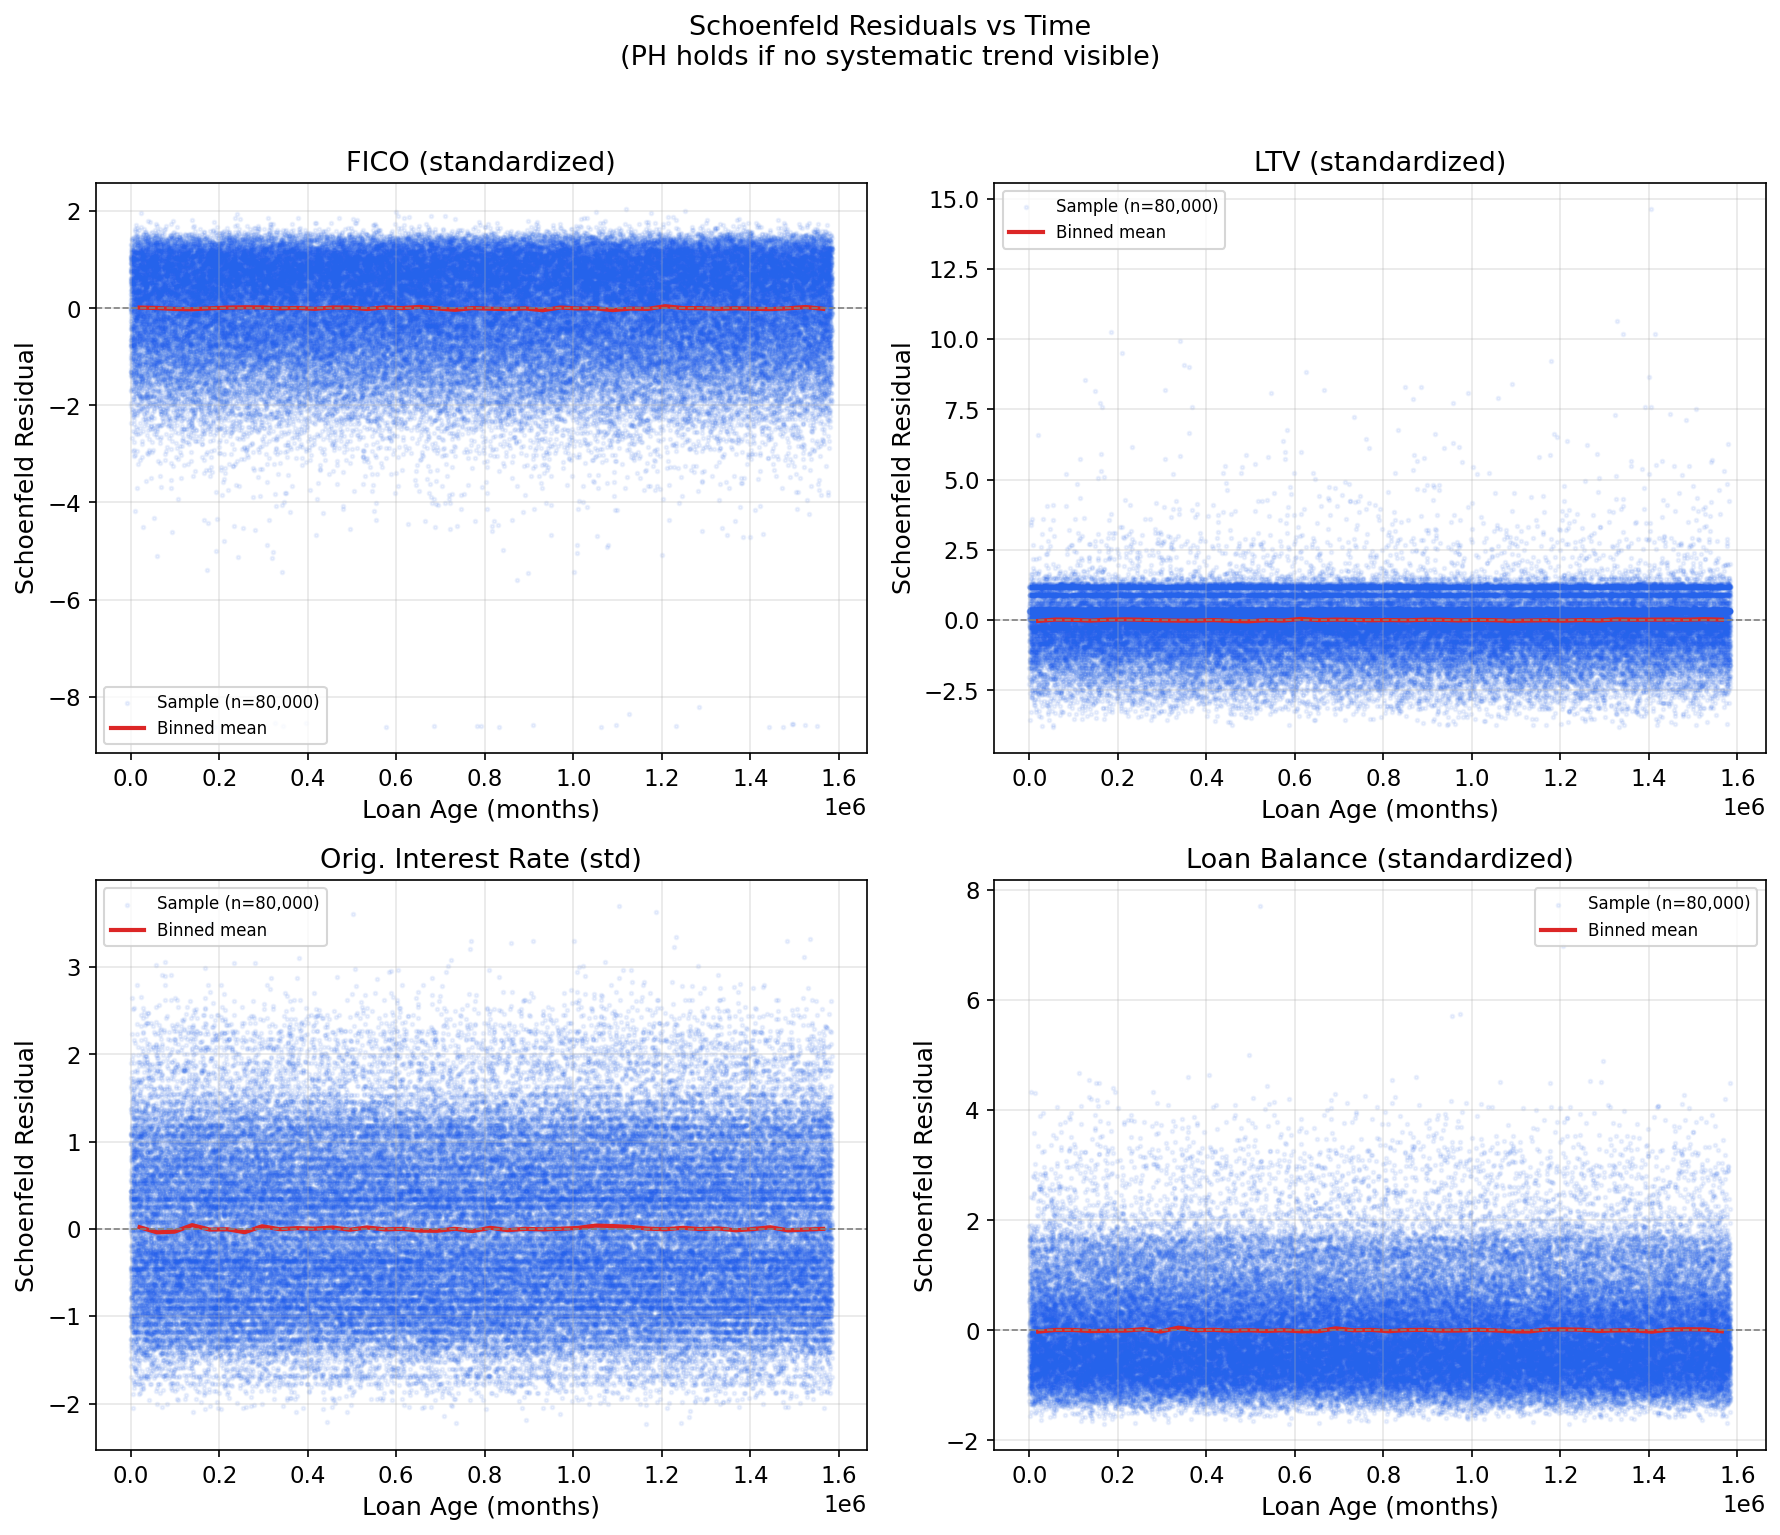
\includegraphics[width=\linewidth]{plots/B_ph_test.png}
        \end{center}
        \column{0.45\textwidth}
        \textbf{Why this matters.}

        \begin{itemize}\itemsep2pt
            \item Standard finding on mortgage data; this is the principal motivation for moving beyond Cox.
            \item PH violation means the hazard ratio for, say, FICO is \emph{not constant} over the life of the loan --- the relative effect of credit quality on prepayment behaves differently at year 1 vs year 5.
            \item Linear models can't represent this. Tree-based and deep models can, by interacting features with loan age.
        \end{itemize}

    \end{columns}

\end{frame}

% ============================================================ Slide 11: Part C setup
\begin{frame}{Part C --- ML Models for Horizon-Specific Prediction}

    \textbf{Reframing.} For each horizon $T \in \{12, 24, 36, 60\}$, we model:
    \[
        P(\text{prepaid by } T \mid X) \quad\text{as a binary classification.}
    \]

    \textbf{Cause-specific exclusions.} Loans with competing termination at $\text{Duration} \leq T$ or right-censored before $T$ are excluded (NaN target), not labeled as 0.

    \textbf{Setup:} 10\% sample, 1.85M train / 597k test, 68 features after one-hot. Same canonical split as Part D.

    \textbf{Four models:}
    \begin{itemize}\itemsep1pt
        \item Logistic Regression ($\ell_2$, internal scaler)
        \item Random Forest (200 trees)
        \item LightGBM (with held-out-validation early stopping)
        \item Cox baseline (lifelines, predict $1 - S(T \mid X)$)
    \end{itemize}

    \textbf{Evaluated:} AUC, Brier, log-loss, accuracy --- per model, per horizon, stratified by vintage and FICO.

\end{frame}

% ============================================================ Slide 12: Part C AUC
\begin{frame}{Part C --- Out-of-Sample AUC}

    \begin{columns}[T,onlytextwidth]
        \column{0.55\textwidth}
        \begin{center}
            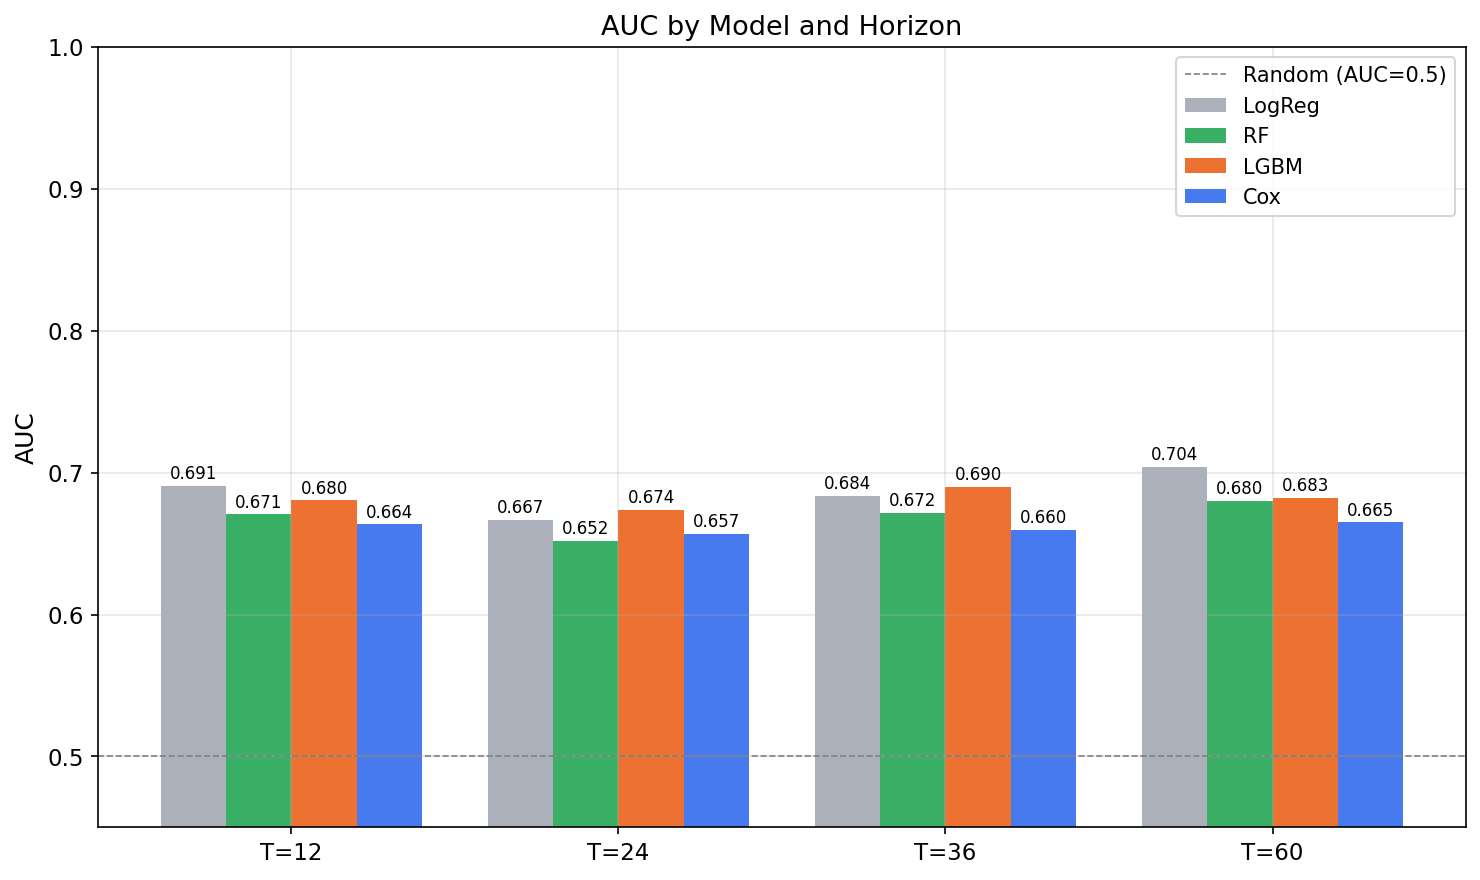
\includegraphics[width=\linewidth]{plots/C_auc_by_horizon.png}
        \end{center}

        \column{0.45\textwidth}
        \small
        \begin{tabular}{lcccc}
            \toprule
            Model  & T=12 & T=24 & T=36 & T=60 \\
            \midrule
            Cox    & 0.66 & 0.66 & 0.66 & 0.67 \\
            RF     & 0.67 & 0.65 & 0.67 & 0.68 \\
            LGBM   & 0.68 & 0.67 & 0.69 & 0.68 \\
            LogReg & 0.69 & 0.67 & 0.68 & 0.70 \\
            \bottomrule
        \end{tabular}

        \vspace{0.7em}
        \normalsize
        \textbf{Observations:}
        \begin{itemize}\itemsep1pt
            \item All four models in the 0.65--0.70 band
            \item LogReg is competitive, even best at T=12 and T=60
            \item Marginal effects in the data are largely linear-additive
            \item Tree models' axis-aligned splits don't unlock much extra signal (yet)
        \end{itemize}

    \end{columns}

\end{frame}

% ============================================================ Slide 13: Part C calibration & lift
\begin{frame}{Part C --- Calibration and Top-Decile Lift}

    \begin{columns}[T,onlytextwidth]
        \column{0.5\textwidth}
        \begin{center}
            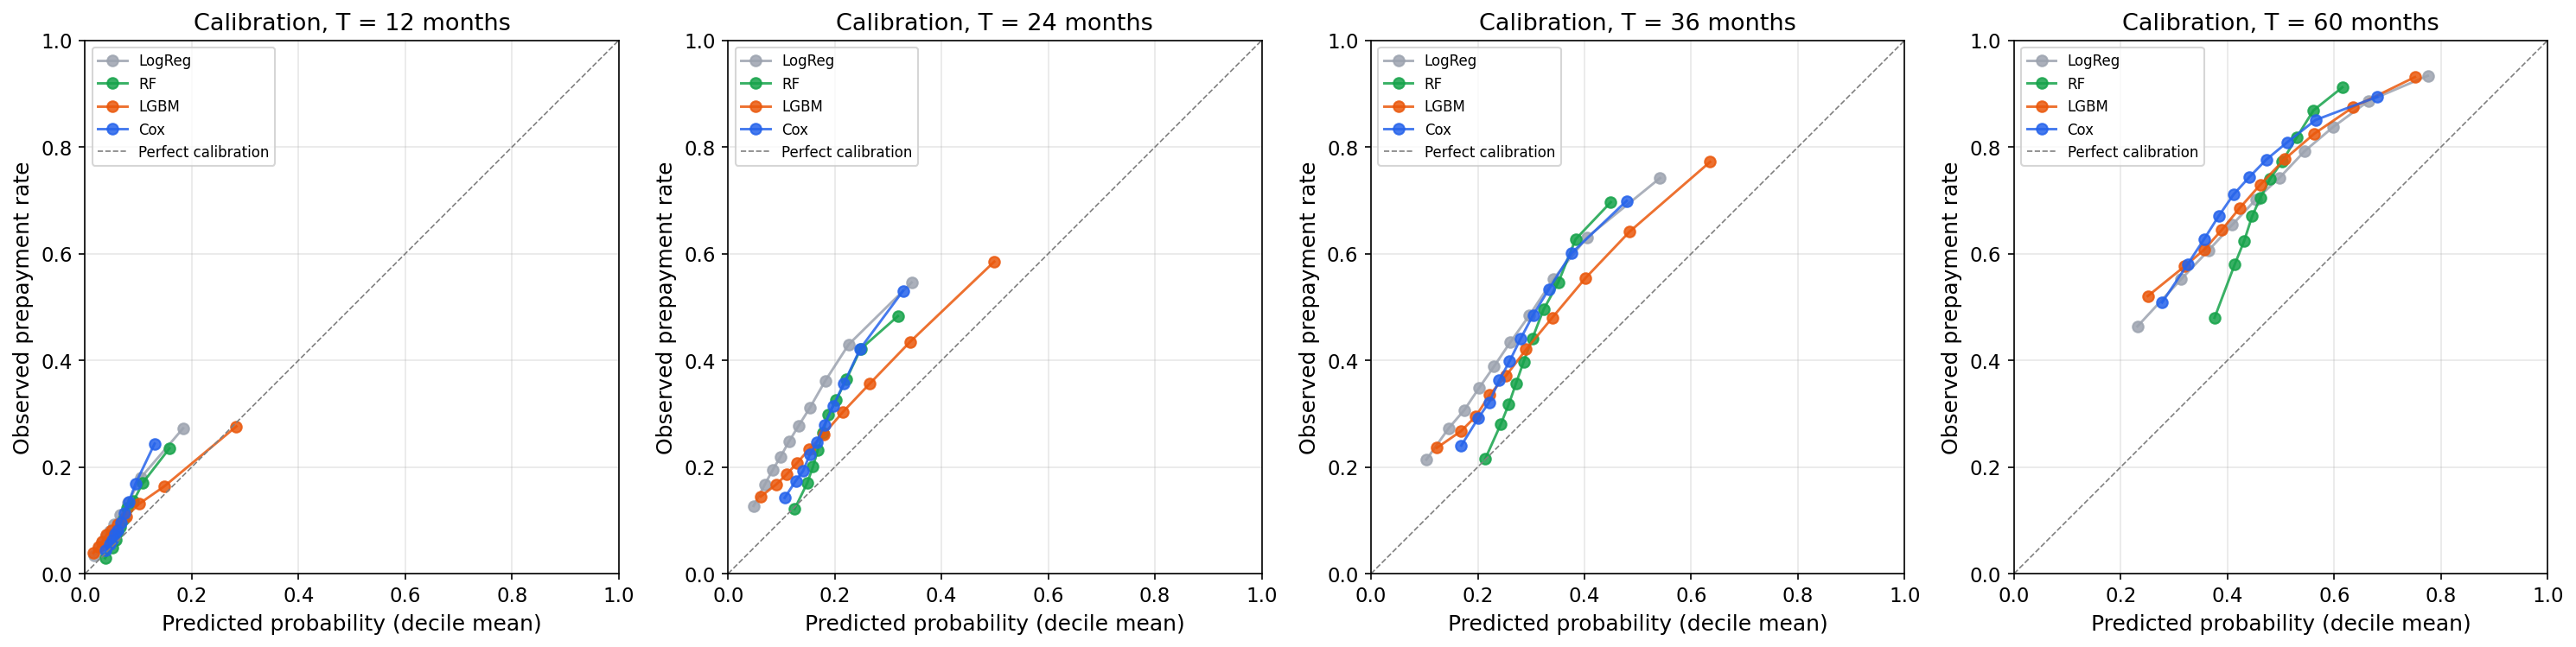
\includegraphics[width=\linewidth]{plots/C_calibration.png}
        \end{center}
        \textbf{Calibration} is reasonable for all models. LightGBM and LogReg sit closest to the diagonal; Cox is slightly under-confident at the high end.

        \column{0.5\textwidth}
        \begin{center}
            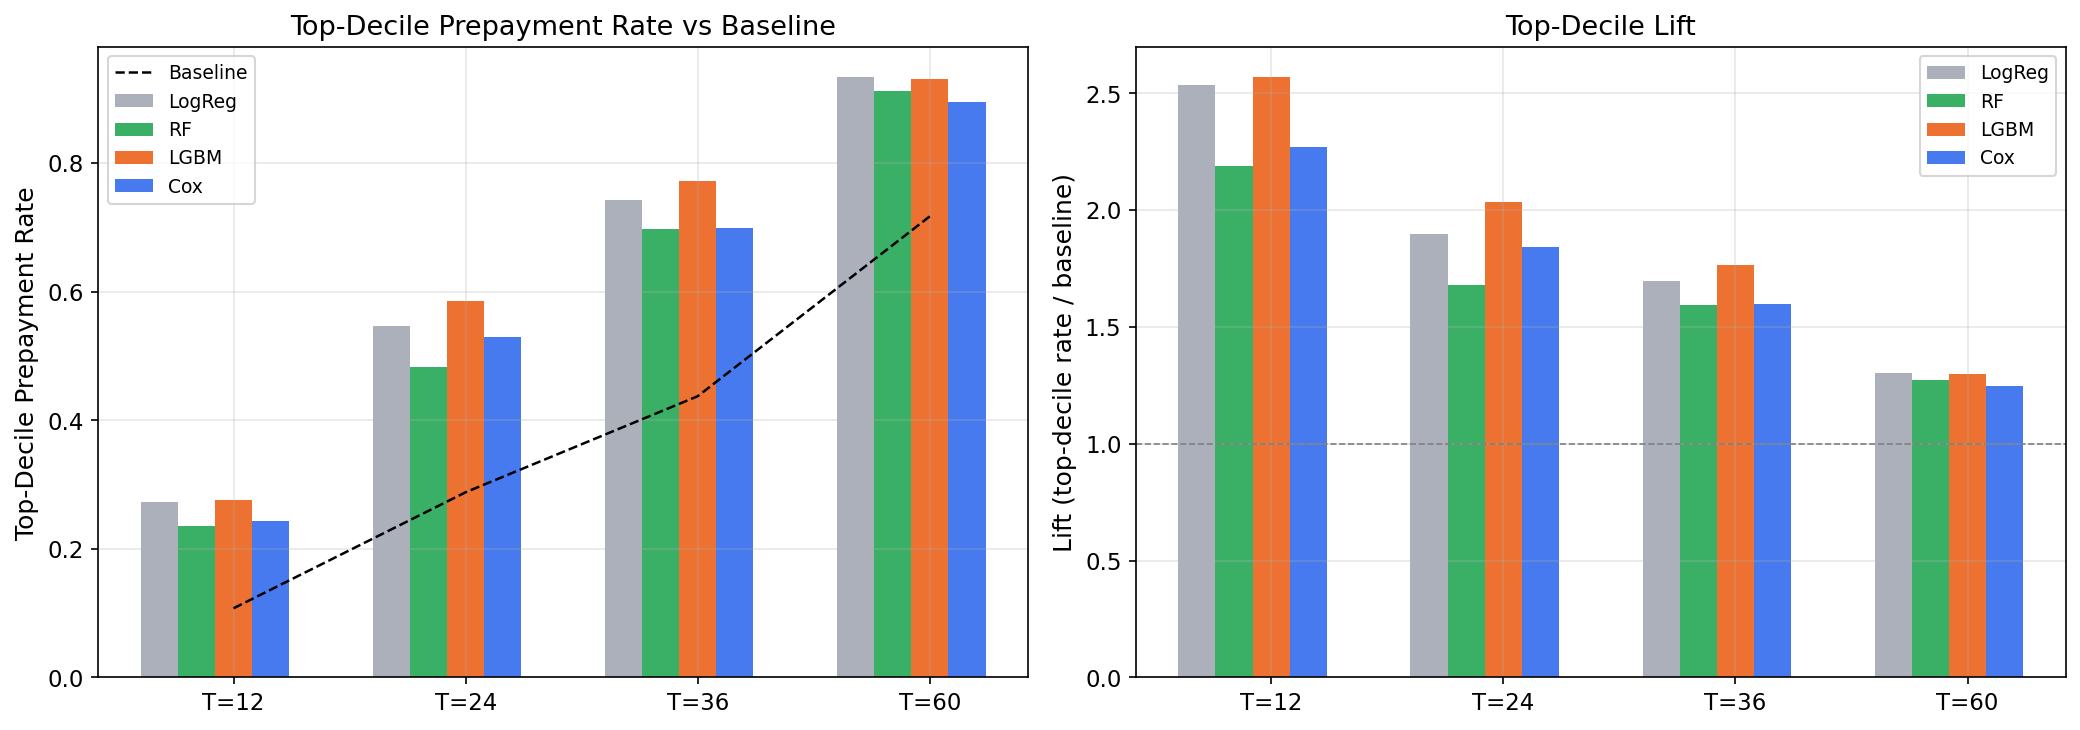
\includegraphics[width=\linewidth]{plots/C_top_decile_lift.png}
        \end{center}

        \textbf{Top-decile lift.} At T=12 the top decile catches 27.6\% prepayments (LightGBM) vs 10.75\% baseline $\to$ \textbf{lift = 2.57$\times$}. Saturates at T=60 because the base rate is already 71.7\%.

    \end{columns}

\end{frame}

% ============================================================ Slide 14: Part D setup
\begin{frame}{Part D --- Deep Cox Architecture and Training}

    \textbf{Model:} $\lambda(t \mid X) = \lambda_0(t) \cdot \exp\!\bigl(f_\theta(X)\bigr)$
    where $f_\theta$ is a feed-forward network.

    \vspace{0.5em}

    \begin{columns}[T,onlytextwidth]
        \column{0.5\textwidth}

        \textbf{Architecture (DeepSurv-standard):}
        \begin{itemize}\itemsep1pt
            \item 3 hidden layers $\times$ 64 ReLU units
            \item Batch normalization, dropout 0.1
            \item No output bias
            \item 13{,}184 parameters
        \end{itemize}

        \textbf{Training (pycox + torchtuples):}
        \begin{itemize}\itemsep1pt
            \item Adam, $\eta = 10^{-3}$, batch 512
            \item Up to 50 epochs, ES patience 8 on val partial-likelihood loss
            \item Mini-batch Cox approximation (risk sets batch-local --- standard pycox / DeepSurv)
            \item Breslow baseline post-fit on full train
        \end{itemize}

        \column{0.5\textwidth}

        \textbf{Linear baseline (D(v) ablation):}
        \begin{itemize}\itemsep1pt
            \item Same pycox infrastructure
            \item \texttt{num\_nodes=[]} $\to$ no hidden layers
            \item 68 parameters (one per feature)
            \item Functionally a SGD-fit classical Cox
        \end{itemize}

        \textbf{Why this is the cleanest possible ablation:} same data, same optimizer, same baseline-hazard estimator $\to$ the only difference is depth.

        \textbf{Runtime:} 17 min Deep + 1 min Linear on CPU.

    \end{columns}

\end{frame}

% ============================================================ Slide 15: Part D ablation
\begin{frame}{Part D --- Linear vs Deep Ablation (D(v))}

    \begin{columns}[T,onlytextwidth]
        \column{0.55\textwidth}
        \begin{center}
            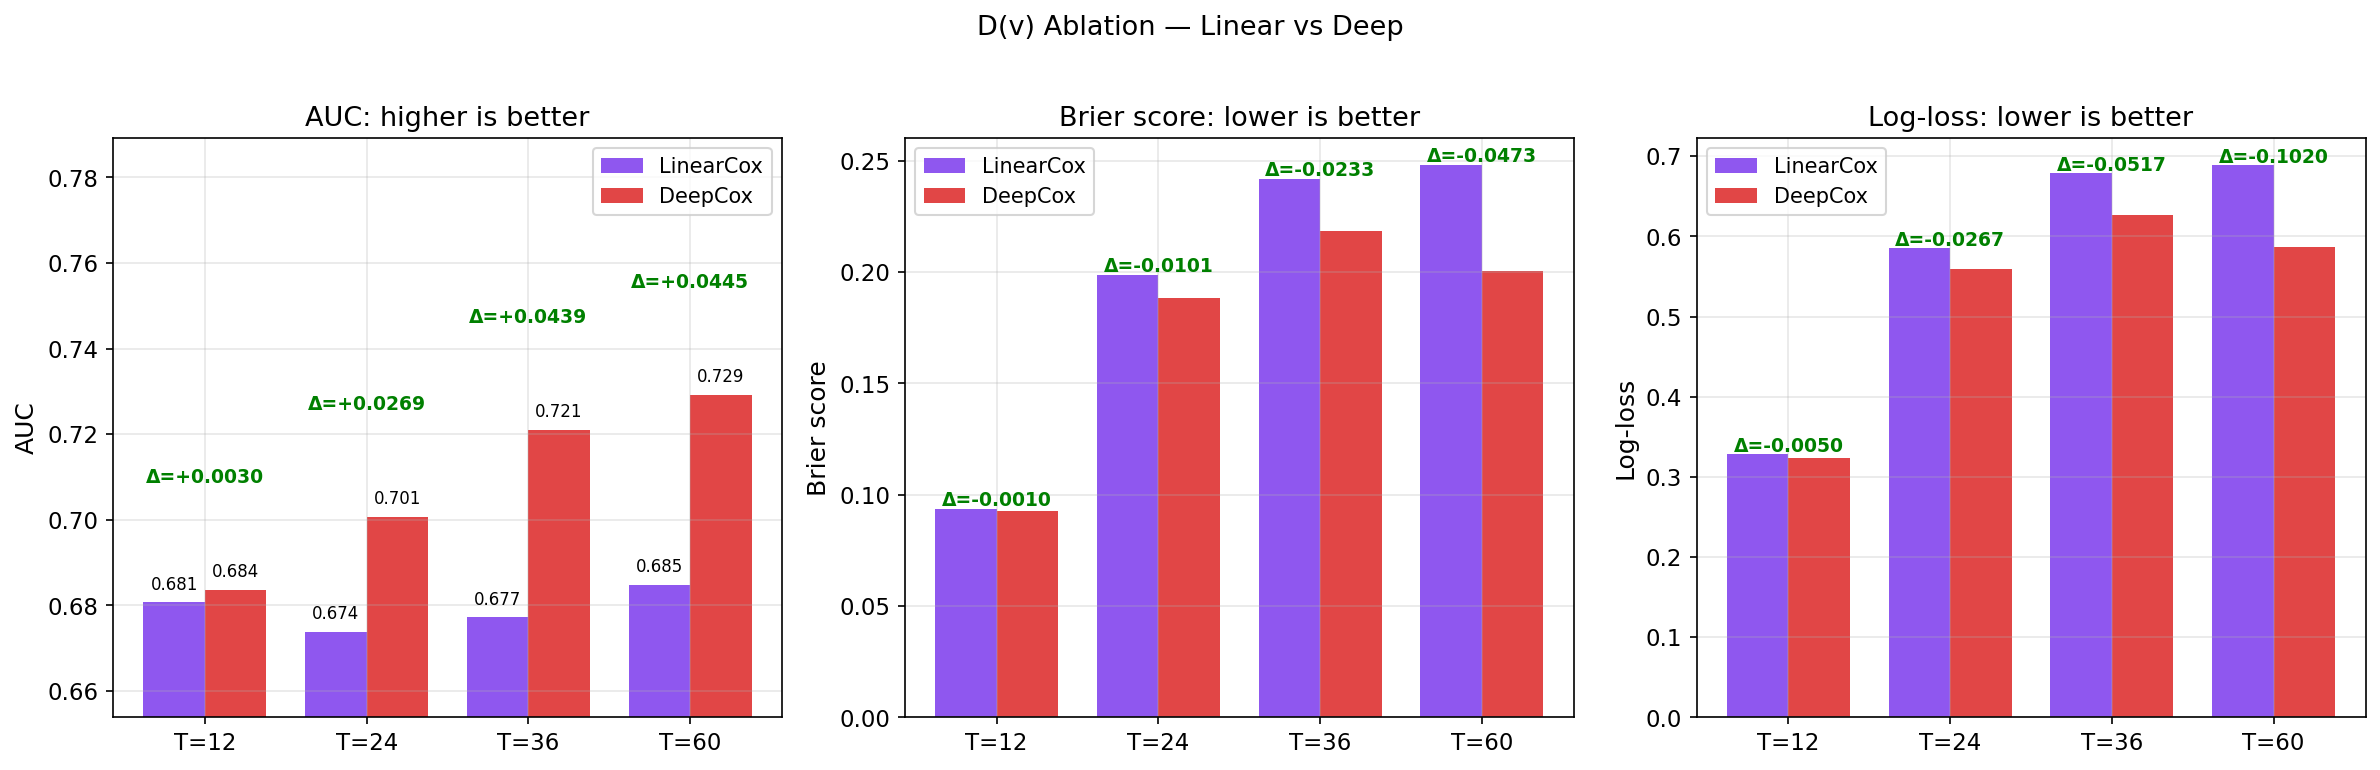
\includegraphics[width=\linewidth]{plots/D_ablation_bars.png}
        \end{center}

        \column{0.45\textwidth}
        \small
        \begin{tabular}{rccc}
            \toprule
            $T$ & Linear & Deep   & $\Delta$AUC                \\
            \midrule
            12  & 0.6807 & 0.6837 & \textcolor{good}{$+0.003$} \\
            24  & 0.6738 & 0.7007 & \textcolor{good}{$+0.027$} \\
            36  & 0.6772 & 0.7211 & \textcolor{good}{$+0.044$} \\
            60  & 0.6848 & 0.7292 & \textcolor{good}{$+0.045$} \\
            \bottomrule
        \end{tabular}

        \vspace{1em}
        \normalsize

        \textbf{The gap widens monotonically with horizon.}

        Sadhwani et al.\ (2021) predicted exactly this --- nonlinear interactions accumulate over the loan's life.

    \end{columns}

\end{frame}

% ============================================================ Slide 16: Part D head-to-head
\begin{frame}{Part D --- Head-to-Head with All Models}

    \begin{columns}[T,onlytextwidth]
        \column{0.55\textwidth}
        \begin{center}
            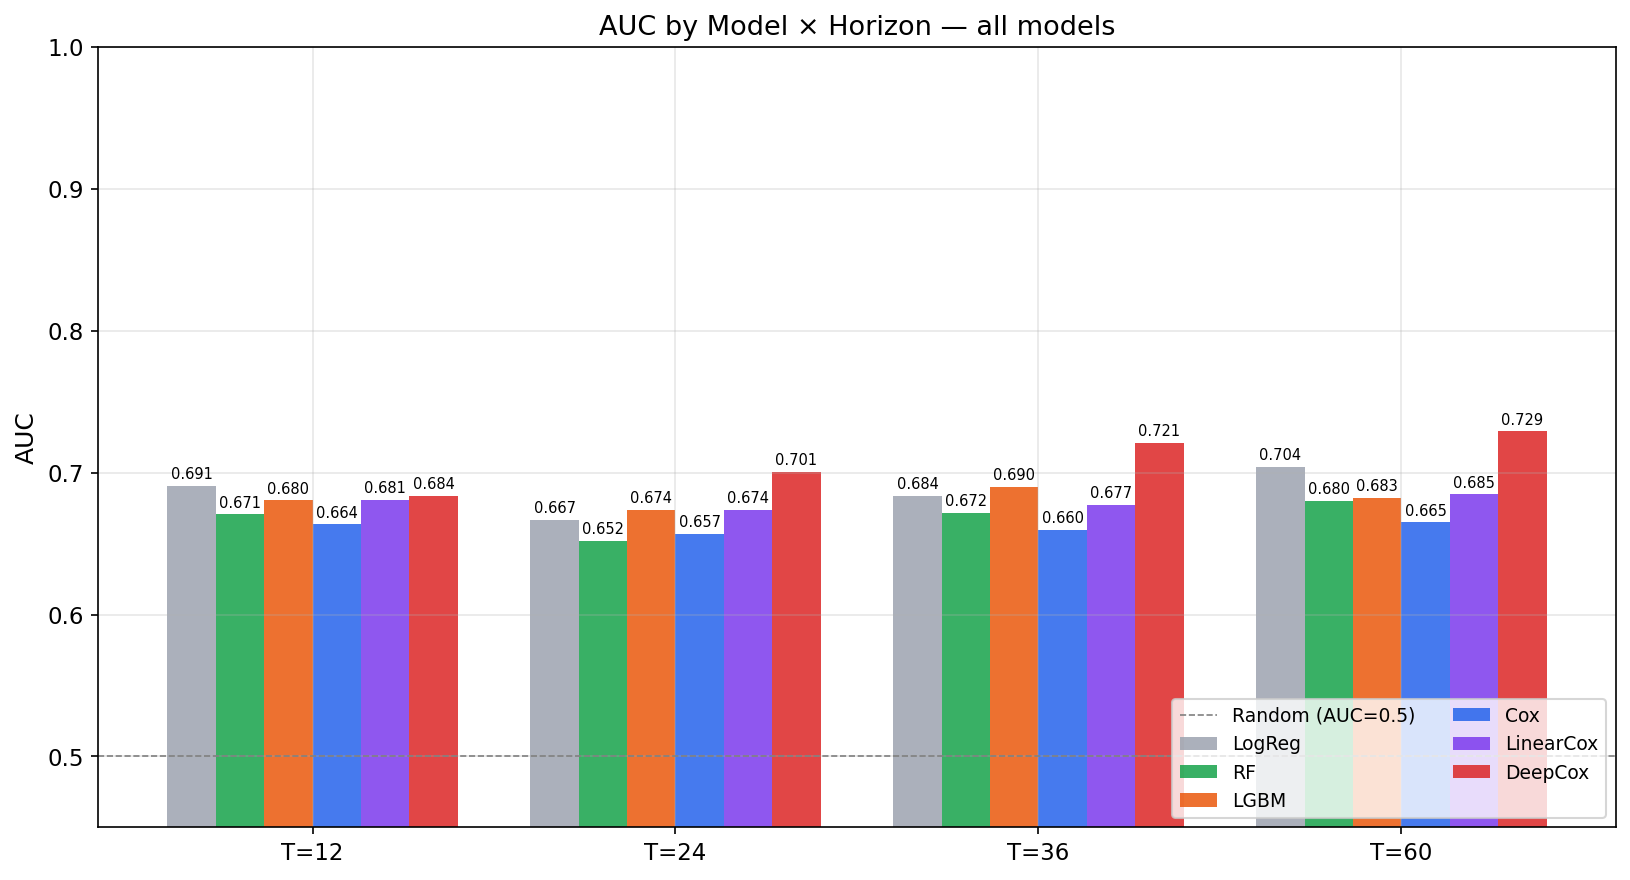
\includegraphics[width=\linewidth]{plots/D_auc_by_horizon.png}
        \end{center}

        \column{0.45\textwidth}
        \small
        \begin{tabular}{lcccc}
            \toprule
            Model            & T=12         & T=24         & T=36         & T=60         \\
            \midrule
            Cox              & .66          & .66          & .66          & .67          \\
            RF               & .67          & .65          & .67          & .68          \\
            LGBM             & .68          & .67          & .69          & .68          \\
            LinearCox        & .68          & .67          & .68          & .68          \\
            LogReg           & .69          & .67          & .68          & .70          \\
            \textbf{DeepCox} & \textbf{.68} & \textbf{.70} & \textbf{.72} & \textbf{.73} \\
            \bottomrule
        \end{tabular}

        \vspace{0.8em}
        \normalsize

        \textbf{DeepCox is best at every horizon $\geq$ 24 months}, often by 0.04--0.05 AUC.

        \textbf{At T=12} LogReg edges it slightly --- short-horizon prepay is dominated by ``easy'' cases (large rate-incentive borrowers).

    \end{columns}

\end{frame}

% ============================================================ Slide 17: Why deep wins at long horizons
\begin{frame}{Why Deep Wins at Long Horizons}

    \textbf{Linear assumption:} the log-hazard is additive in covariate effects.
    $$
        \log \lambda(t \mid X) \;=\; \log \lambda_0(t) + \beta_1 x_1 + \beta_2 x_2 + \cdots
    $$
    A loan with high rate \emph{plus} high FICO \emph{plus} low LTV experiences a hazard that is the product of independently-acting multipliers.

    \vspace{0.4em}

    \textbf{Reality:} prepayment incentive is \emph{joint} in covariates.

    The refinancing decision conditional on still being alive at $T{=}36$ depends on the borrower's current FICO, balance, rate environment they would face refinancing into --- and these interact non-trivially.

    \vspace{0.4em}

    \textbf{At long horizon, more interaction paths matter.} The deep network captures them; the linear model collapses them. Hence the widening gap.

    \vspace{0.4em}

    \textbf{At T=12} only borrowers with very strong, singular incentive have prepaid. Easy cases for any model.

    \vspace{0.6em}

    \begin{center}
        \textcolor{accent}{\textit{Same conclusion as Sadhwani--Giesecke--Sirignano (2021) on the much larger CoreLogic dataset.}}
    \end{center}

\end{frame}

% ============================================================ Slide 18: Calibration & top-decile lift D
\begin{frame}{Part D --- Calibration and Top-Decile Lift}

    \begin{columns}[T,onlytextwidth]
        \column{0.5\textwidth}
        \begin{center}
            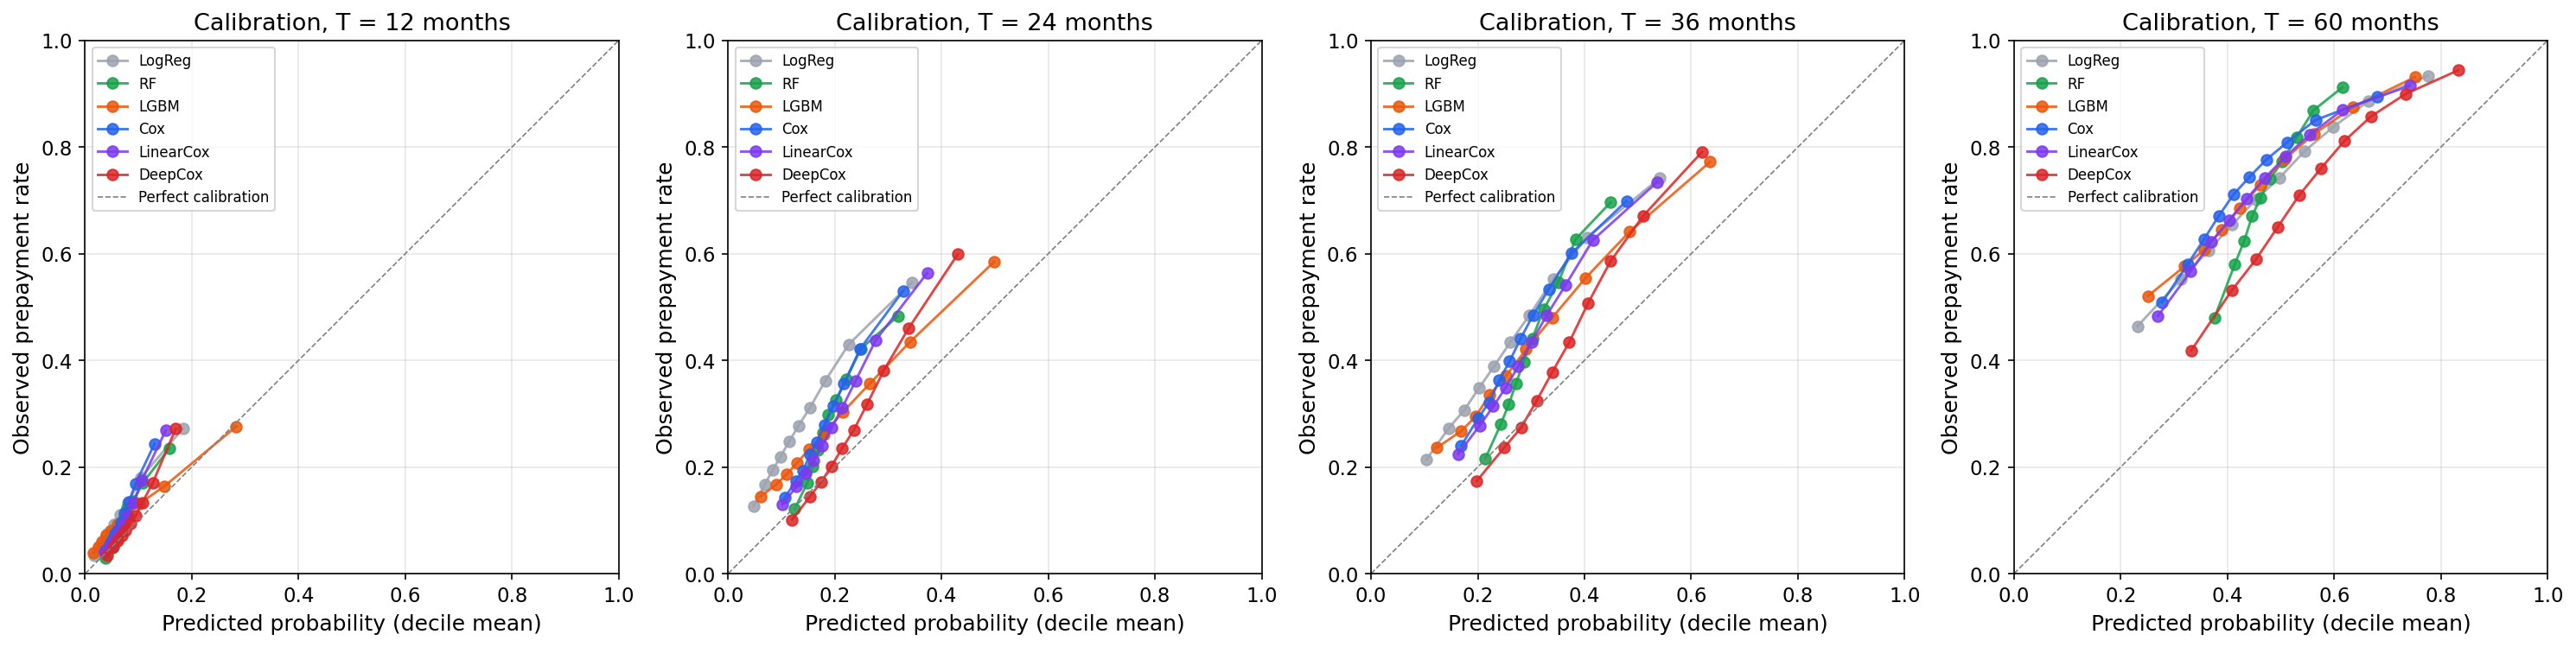
\includegraphics[width=\linewidth]{plots/D_calibration.png}
        \end{center}
        \textbf{Calibration.} DeepCox sits close to the diagonal at all horizons. LinearCox slightly under-confident.

        \column{0.5\textwidth}
        \begin{center}
            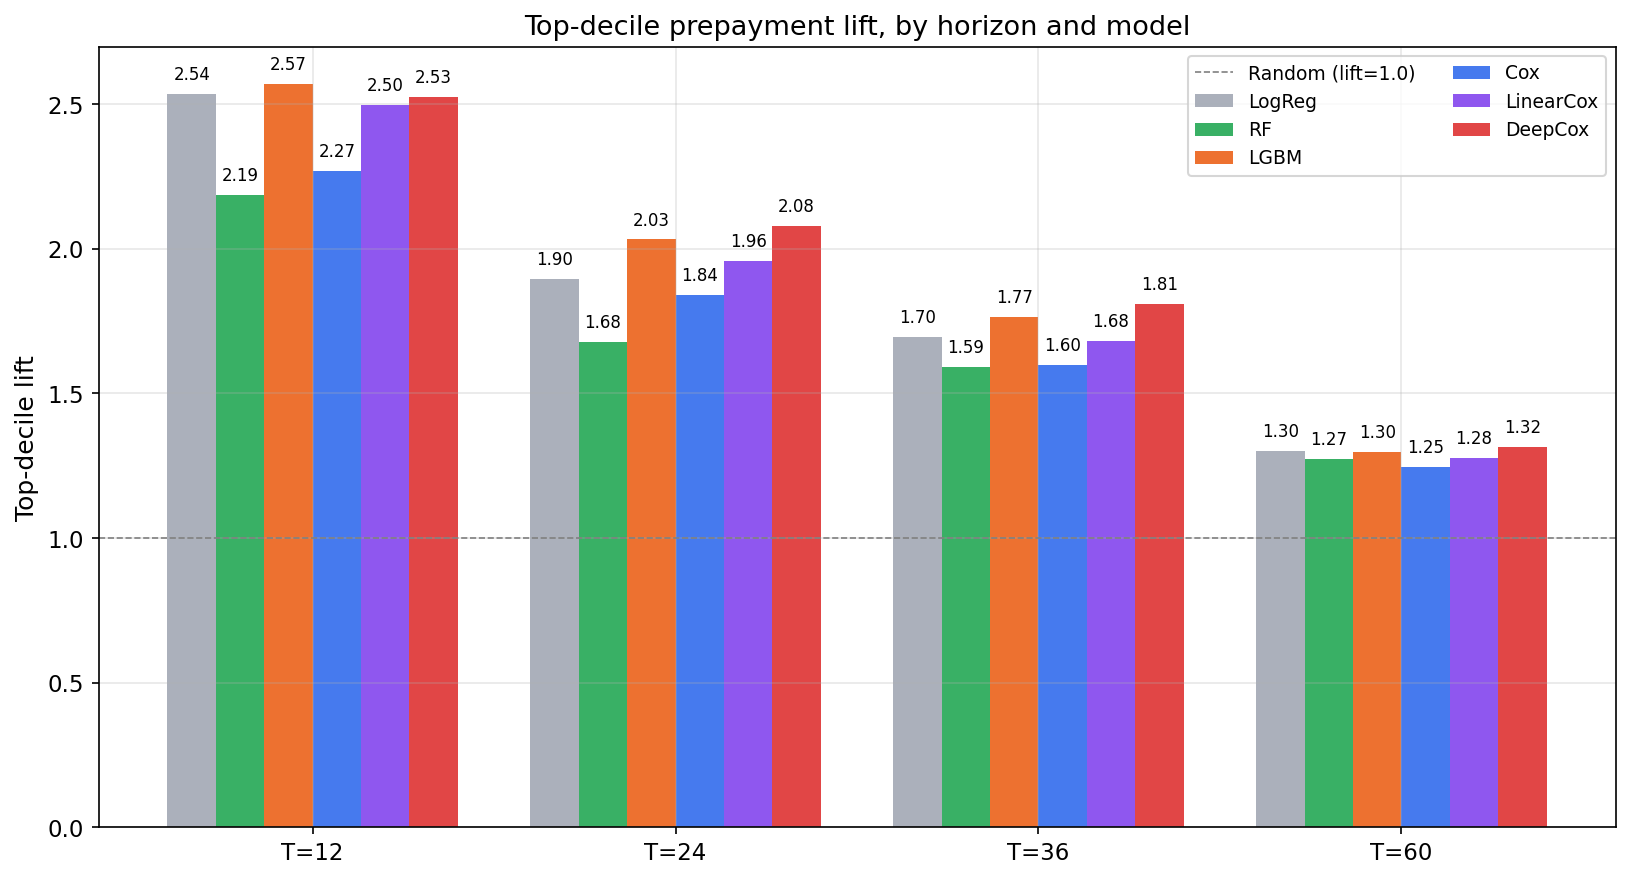
\includegraphics[width=\linewidth]{plots/D_top_decile_lift.png}
        \end{center}

        \textbf{Top-decile lift.} At moderate horizons (T=24, T=36) DeepCox catches more positives:
        \begin{itemize}\itemsep0pt
            \small
            \item T=24: DeepCox 2.08$\times$ vs LGBM 2.03$\times$ vs LogReg 1.90$\times$
            \item T=36: DeepCox 1.81$\times$ vs LGBM 1.77$\times$
        \end{itemize}

    \end{columns}

\end{frame}

% ============================================================ Slide 19: Limitations
\begin{frame}{Limitations and Future Work}

    \textbf{What this study didn't do:}
    \begin{enumerate}\itemsep2pt
        \item \textbf{Time-varying covariates.}  Macro covariates are joined at origination only. A truly dynamic Cox would join the current rate environment, current LTV (HPI-updated), current unemployment --- but requires the loan-month panel ($\sim$3.5B rows).
        \item \textbf{Competing risks.}  We use cause-specific censoring for prepayment. A multi-output network jointly modeling prepay, default, and survival (Fine--Gray subdistribution hazards or multi-state) would be more complete.
        \item \textbf{Mini-batch Cox sensitivity.}  Risk sets are batch-local; a sensitivity check across batch sizes 256/512/1024/2048 would strengthen the conclusions. Standard practice in DeepSurv literature, but worth verifying.
        \item \textbf{Distribution shift.}  Vintage-based train/test split means the test set sees a different rate environment than train. Honest --- but the absolute AUCs reflect distribution shift, not just model capacity.
    \end{enumerate}

    \textbf{Natural extensions:}
    \begin{itemize}\itemsep1pt
        \item Time-dependent covariates via loan-month panel
        \item Recurrent or attention-based survival models
        \item Interest-rate scenario analysis using the trained model
    \end{itemize}

\end{frame}

% ============================================================ Slide 20: What we learned
\begin{frame}{Key Takeaways}

    \begin{enumerate}\itemsep4pt

        \item \textbf{Mortgage prepayment is not a linear-in-covariates process.}
              Schoenfeld test rejects PH for 12/15 covariates. The cleanest evidence:  Linear vs Deep ablation at fixed everything-else.

        \item \textbf{Deep Cox AUC = 0.729 at T=60} vs 0.685 linear baseline ($\Delta = +0.045$).  Not a small effect.  And it grows with horizon.

        \item \textbf{Tree models don't close the gap.}  LightGBM tops out at 0.68--0.69; Random Forest below that.  Suggests interactions are smooth-and-multivariate (good for MLPs) rather than coarse-and-axis-aligned (good for trees).

        \item \textbf{Logistic regression is surprisingly competitive at the short end} (T=12).  When prepayment is concentrated in a tail of obvious refi candidates, marginal effects suffice.

        \item \textbf{Vintage-macro covariates earn their place.}  Cox concordance jumps from 0.626 to 0.643 just from joining FRED data at origination.

        \item \textbf{Deep Cox is well-calibrated} --- rare for a survival NN, attributable to the structural Breslow baseline rather than direct probability fitting.

    \end{enumerate}

\end{frame}

% ============================================================ Slide 21: Code statistics & process
\begin{frame}{Code Statistics and Process Notes}

    \begin{columns}[T,onlytextwidth]
        \column{0.50\textwidth}
        \textbf{Codebase:}

        \vspace{0.5em}

        \textbf{Subsamples and splits:}
        \scriptsize
        \begin{tabular}{p{0.22\linewidth}p{0.70\linewidth}}
            Part A & Full 31.69M-loan population; no sampling.                                        \\
            Part B & 5\% Cox sample: 1.58M loans, 1.08M events; PH diagnostic uses 158k rows.         \\
            Part C & Shared 10\% universe: 1.85M train / 597k test; 68 one-hot features.              \\
            Part D & Same C/D split; 10\% validation carve: 1.66M inner train / 185k val / 597k test. \\
        \end{tabular}

        \column{0.50\textwidth}
        \textbf{Engineering notes:}
        \begin{itemize}\itemsep2pt
            \small
            \item \textbf{Memory.} Polars survival-table build, sentinel cleaning, and float32 kept peak around 10 GB.

            \item \textbf{Reproducibility.} One \texttt{canonical\_split.parquet}; train-only encoders/scalers persisted and reused by Parts C/D.

            \item \textbf{Leakage fixes.} Cross-AI review caught encoder fitting before split and Part D validation carving after standardization; both corrected.

            \item \textbf{Session boundaries.} \texttt{utilities.py} acted as the API contract across multiple coding sessions.

            \item \textbf{Model plumbing.} Thin pycox-to-lifelines adapter enabled Deep/Linear Cox vs classical Cox comparison.
        \end{itemize}
    \end{columns}

\end{frame}

% ============================================================ Slide 22: Thank you
\begin{frame}[plain]
    \vspace*{1.5em}
    \begin{center}
        {\Huge \textbf{Thank you}}

        \vspace{1.5em}

        {\Large Questions?}

        \vspace{2.5em}

        \begin{minipage}{0.7\textwidth}
            \centering
            \small
            \textbf{Reproducibility}\\[0.3em]
            Six scripts + four notebooks, $\approx$ 50 min CPU runtime.\\
            All encoders, scalers, and seeds persisted.

            \vspace{1.5em}

            \textbf{References}\\[0.3em]
            Sadhwani, Giesecke, Sirignano (2021), \emph{J.\ Financial Econometrics} \\
            Katzman et al.\ (2018), DeepSurv, \emph{BMC Medical Research Methodology} \\
            Kvamme et al.\ (2019), pycox, \emph{JMLR} \\
            Davidson-Pilon (2019), lifelines, \emph{JOSS}
        \end{minipage}
    \end{center}
\end{frame}

\end{document}
